\documentclass[english,12pt,a4paper]{book}
\usepackage[T1]{fontenc} % In case we want special characters
\usepackage[utf8]{inputenc} % We are all writing in UTF-8

\usepackage[numbers]{natbib} % We need to tweak our referencing a bit.
\usepackage{appendix} % Fixes formatting of appendices
\usepackage[printonlyused]{acronym} % Package to handle the acronym list
\usepackage{graphicx} % We *may* use images
\graphicspath{{images/}} % and it is clean to put them in a separate dir
\usepackage{hyperref} % Internal and external links is nice
\hypersetup{pdfborder=0 0 0} % ..especially without red borders

% Packages and settings for code listings
\usepackage{listings}
\usepackage{caption}
\usepackage{upquote}
\usepackage{xcolor}
\DeclareCaptionFont{white}{\color{white}}
\DeclareCaptionFormat{listing}{\colorbox{gray}{\parbox{\textwidth}{#1#2#3}}}
\captionsetup[lstlisting]{format=listing,labelfont=white,textfont=white}
\lstset{
language=Python,
keywordstyle=\bfseries\ttfamily\color[rgb]{0,0,1},
identifierstyle=\ttfamily,
commentstyle=\color[rgb]{0.133,0.545,0.133},
stringstyle=\ttfamily\color[rgb]{0.627,0.126,0.941},
showstringspaces=false,
basicstyle=\small,
numberstyle=\footnotesize,
numbers=left,
stepnumber=1,
numbersep=10pt,
tabsize=2,
breaklines=true,
prebreak = \raisebox{0ex}[0ex][0ex]{\ensuremath{\hookleftarrow}},
breakatwhitespace=false,
aboveskip={1.5\baselineskip},
columns=fixed,
upquote=true,
extendedchars=true,
frame=bottomline,
inputencoding=utf8
}

% Set equal margins on book style
% \usepackage{layout} % Use \layout to print out the margins (debug)
\usepackage{geometry}
\geometry{bindingoffset=1cm}

\author{Eirik Haver \and Pål Ruud}
\title{Project assignment - Tahoe-LAFS with SHA-3 candidates}
\date{\today}

\begin{document}

% Latex-versjon av ITEM rapportmal.
% Lagd av <lasse.karstensen@gmail.com>, desember 2009.
% Lisens: public domain. 
%
\begin{titlepage}
\begin{center}
\textsc{NORWEGIAN UNIVERSITY OF SCIENCE AND TECHNOLOGY\\
FACULTY OF  INFORMATION TECHNOLOGY, MATHEMATICS AND ELECTRICAL ENGINEERING} \\
\vspace{0.5cm} 
% crop-et fra http://www.ntnu.no/infoavdelingen/selvhjelp/logoer/ntnu/NTNU_engelsk_RGB.png

\includegraphics[scale=0.5]{NTNU-logo} \\

\vspace{1.0cm}
{\Huge{PROJECT ASSIGNMENT}}
\vspace{1.0cm}

\begin{tabular}{ p{4cm} p{11cm}}

Students' name:	& Eirik Haver and Pål Ruud \\
Course: & TTM13 \\
Title: & Experimenting with SHA-3 candidates in Tahoe-LAFS \\
%\vspace{1cm}
Description: & \\
\end{tabular}
{\small{\begin{tabular}{p{15cm}}
\vspace{0.2cm}

Tahoe-LAFS is a Free Software/Open Source decentralized data store. It
distributes your filesystem across multiple servers, and even if some of the
servers fail or are taken over by an attacker, the entire filesystem continues
to work correctly and to preserve your privacy and security.
\\\\
One of the basic security components used in Tahoe-LAFS is the cryptographic
hash function SHA-256.
\\\\
In the light of the worldwide SHA-3 hash competition, this task is about
making a reproducible, automated benchmark which shows how the performance of
Tahoe-LAFS is affected by the performance of the different SHA-3 candidate hash
functions. Before any testing can be done, Python bindings to the C
implementations of the SHA-3 candidates have to be made, since Tahoe-LAFS is
written in the Python programming language.
\\\\
\end{tabular}  }}

\begin{tabular}{ p{4cm} p{11cm}}
Deadline: & 2010-12-xx \\
Submission date: & 2010-12-xx \\
Department: & Department of Telematics \\
Supervisor: & Danilo Gligoroski \\\\
\end{tabular}
\vspace{0.5cm}

Trondheim, \today 

\vspace{0.4cm}
\line(1,0){150} \\
Danilo Gligoroski, NTNU/ITEM. 

\end{center}
\end{titlepage}


\pagestyle{empty}

\chapter*{Abstract}
\addcontentsline{toc}{chapter}{Abstract}
\pagestyle{plain}
\pagenumbering{Roman}
\setcounter{page}{1}

\chapter*{Preface}
\addcontentsline{toc}{chapter}{Preface}

\tableofcontents

\addcontentsline{toc}{chapter}{\listfigurename} % Manually add to ToC
\listoffigures

\addcontentsline{toc}{chapter}{\listtablename}
\listoftables

\chapter*{Acronyms}
\addcontentsline{toc}{chapter}{Acronyms}

\begin{acronym}
\acro{AES}{Advanced Encryption Standard}
\acro{API}{Application programming interface}
\acro{CEB}{Capability Extension Block}
\acro{Distutils}{Python Distribution Utilities}
\acro{FEC}{Forward Error Correction}
\acro{GCC}{GNU Compiler Collection}
\acro{KAT}{Known Answer Test}
\acro{LAFS}{Least-Authority Filesystem}
\acro{NIST}{National Institute of Standards and Technology}
\acro{RAM}{Random Access Memory}
\acro{RAID}{Redundant Array of Independent Disks}
\acro{SHA}{Secure Hash Algorithm}
\acro{SSE2}{Streaming SIMD Extensions 2}
\acro{SSSE3}{Supplemental Streaming SIMD Extensions 3}
\acro{SUPERCOP}{System for Unified Performance Evaluation Related to
Cryptographic Operations and Primitives}
\acro{UEB}{URI Extension Block}
\end{acronym}

%**************************************%
\chapter{Introduction}
%**************************************%
\pagenumbering{arabic}
\setcounter{page}{1}

Thorough problem description. \\
Stepwise, what will we actually do?

\section{Method}

Technical procedure, Cython, two persons, test environment, how we test,
GitHub?

\section{Scope and objectives}

Should we include this?

\section{Outline}

What follows in this document, chapter by chapter

%**************************************%
\chapter{Background technologies}
%**************************************%
% FIXME: Find new and better title

\section{Cryptographic Hash Functions}

A cryptographic hash function is a deterministic mathematical procedure which
takes an arbitrary block of data and outputs a fixed-size bit string. The output
is referred to as the hash value, message digest or simply digest.
Another property of a cryptographic hash function is that the smallest change in
the input data (e.g. one bit) should completely change the output of the hash
function. In other words it should be infeasible to find the reverse of a
cryptographic hash function \cite[p. 335]{stallings}. It should also be infeasible to
find two blocks of data which produce the same hash value (a \emph{collision}).

\subsection{NIST SHA-3 Competition}
The \ac{SHA} version 3 is a coming standard set to supersede the current
standards that the \ac{SHA}-1 and the \ac{SHA}-2 family has become. The hash
function that will be known as \ac{SHA}-3 will be decided by the \ac{NIST} and
chosen between the submitted contestants to the \ac{NIST} hash competition.
At the time of writing, the current status of the competition is officially
called Round 2, with 14 of 64 candidates having ``survived'' Round 1
\cite{s_fedreg}.

\subsubsection{\ac{NIST} evaluation criteria for \ac{SHA}-3}

\label{sec:lengthextension}
\paragraph{Security.} The most important criteria for the SHA-3
candidates\cite{s_nistround2} is security. The full description of security
criteria are mentioned in \cite{s_fedreg}, however the most noteworthy criterion
in regards to Tahoe-\ac{LAFS} is that \ac{SHA}-3 candidates are required to have
resistance against length-extension attacks. Both \ac{SHA}-1 and the \ac{SHA}-2
family are vulnerable to this kind of attack, and thus requires
Tahoe to run the algorithm twice, as described by \citet{schneier}.

\paragraph{Cost and Performance.} Cost and Performance are considered to be the
2nd most important criterion. The absolute minimum for performance is that the
SHA-3 candidate should be faster than the functions in the \ac{SHA}-2 family.
Cost is a measure of how much memory an implementation requires in software,
both the implementation itself and the use of \ac{RAM} during runtime. Another
measure of cost is how many logic gates it takes to implement the function in
hardware.

\paragraph{Algorithm and implementation characteristics.} By this 3rd criteria,
\ac{NIST} emphasizes that algorithms with greater flexibility will be given
preference over other algorithms \cite{s_nistround2}. By flexible, they imply
the possibility of the function to run efficiently on a variety of platforms,
and to use parallelism and instruction set extensions. Another key point of a
flexible hash function is that it should have a simple and elegant design to
encourage understanding, analysis and design confidence.

\subsubsection{\ac{NIST} \ac{SHA}-3 \ac{API}}
\ac{NIST} required that every submission conform to a specified
\ac{API}\cite{s_fedreg}. The \ac{API} is specified at \cite{s_nistapi} and in
shortness it requires every candidate to implement four functions.

\begin{verbatim}
HashReturn Init(hashState *state, int hashbitlen);
HashReturn Update(hashState *state, const BitSequence *data, 
    DataLength databitlen);
HashReturn Final(hashState *state, BitSequence *hashval);
HashReturn Hash(int hashbitlen, const BitSequence *data, 
    DataLength databitlen, BitSequence *hashval);
\end{verbatim}

The Init() function basically sets up the internal state of the function, to
make it ready to start processing real data. The Update() function is used to
provide the actuall data to the hash function. The Final() function should be
called when all necessary data has been gived through Update(), it will then
finish the hash function and provide the digest. The Hash() function basically a wrapper
for doing a call to the three other functions.

HashReturn is an enum representing that an operation either succeded (0) or
went wrong. The BitSequence is a representation of an array of bytefields and
DataLength represents the size in bits of the data provided.

\subsection{\ac{SUPERCOP}}
% TODO: Mention that some SUPERCOP candidates are missing UPDATE-functionality.
\ac{SUPERCOP} is a toolkit developed by VAMPIRE lab for measuring performance
of cryptographic software \cite{s_supercop}. In relation to hash functions
\ac{SUPERCOP} measures the following:

\begin{itemize}
    \item Time to hash a very short packet of data.
    \item Time to hash a typical-size Internet packet.
    \item Time to hash a long message.
    \item Length of the hash output.
\end{itemize}

The Round 2 \ac{SHA}-3 candidates are all included in the toolkit, with a number
of different optimizations for each candidate. Optimizations range from
32-/64-bit specific implementations, the use of extended instruction sets such
as \ac{SSE2} and \ac{SSSE3}, optimizations for different number of cores and
others. The toolkit will also try different compiler optimizations to get the
best results possible for each function.
% TODO: Insert image to visualize the forest of different implementations.

The benchmarking results for the \ac{SUPERCOP} toolkit of the \ac{SHA}-3
candidates and \ac{SHA}-2 functions on a number of different plattforms and
architectures are available at
\footnote{\url{http://bench.cr.yp.to/results-sha3.html}}
% TODO: Link to appendix with tahoe04 SUPERCOP results.

\subsubsection{\ac{SUPERCOP} \ac{API}}
\ac{SUPERCOP} specifies an \ac{API} which all submitted implementations must
conform to\cite{s_supercopapi}. This \ac{API} specifies the naming and
organization of files, and that a submission must include a function
crypto\_hash() which is similar to the function Hash() in the \ac{NIST} \ac{SHA}-3
\ac{API}. The only difference beeing the naming of datatypes and that the
crypto\_hash() function does not need an input of how long the output of the
hash function should be. Instead double or different submissions are used for
different output lengths.

\begin{verbatim}
int crypto_hash(unsigned char *out, const unsigned char *in,
    unsigned long long inlen)
\end{verbatim}

\section{Tahoe-LAFS}
%What is it, how/where are hash functions used, Python, pycryptopp
%comparison with RAID-6, mutable/immutable?

The Tahoe \ac{LAFS} is a system for secure,
distributed data storage. Files are encrypted client side, then
split up, before each part is sent to other nodes in the grid, as depicted in
figure \ref{fig:tahoeinsertion}. The integrity and confidentiality of the files
are guaranteed by the algorithms used on the client, and is independent of the
storage servers, which may be operated by untrusted people. This is defined as
\emph{provider-independent security} \cite{t_tahoe}.

\begin{figure}[h!]
    \centering
    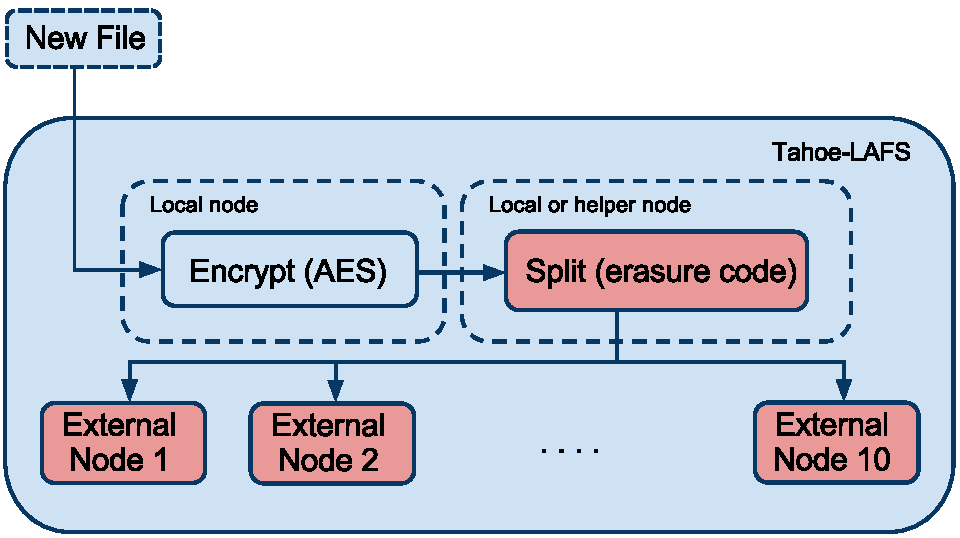
\includegraphics[width=0.9\columnwidth]{Tahoe-newfile.pdf}
    \caption{Tahoe-LAFS: Insertion of new file}
    \label{fig:tahoeinsertion}
\end{figure}

Tahoe was originally developed with funding from the former commercial web
backup service provider Allmydata, but is now a stand-alone Open
Source\footnote{GNU General Public License (GPL) version 2} project
\cite{t_ars}.  It is written in the Python programming language with the Twisted
framework, and can run on Windows, Mac OSX, Linux, Solaris and more.

\subsection{Architecture}

Tahoe has a three layer architecture: the key-value store, the filesystem, and
the application \cite{t_tahoe}.

The \textbf{key-value store}, or the ``capability-data bytes'' store, is the
lowest layer and is implemented by a grid of Tahoe-LAFS storage servers. Data is
kept on the storage servers in the form of ``shares'', which are encrypted and
encoded parts of files. Capabilities are short ASCII strings, containing
information on where to \emph{find} a file, and how to \emph{verify} it.
Nodes in the grid learn about each other through an ``introducer'', which
roughly relates to a tracker in the BitTorrent\footnote{See
\url{http://www.bittorrent.org/beps/bep\_0003.html}} protocol.

The \textbf{filesystem} layer is responsible for mapping human-meaningful
pathnames to pieces of data. Each directory contains a table of capabilities
for its children, i.e. subdirectories or files. Two forms of capabilities is
available for each file, read-only and read-write, and these can be shared to
provide shared/published directory structures with friends.

Since it is not practical for users to remember strings containing random
characters, the \textbf{application} layer is used for providing a user-friendly
interface to the directories and files.

\paragraph{File types.}

There are two kinds of files in the Tahoe-\ac{LAFS} -- \textbf{immutable} and
\textbf{mutable} files. An immutable file is created exactly once, i.e. it
cannot be modified, and can be read repeatedly. Mutable files can be modified,
and everyone who has access to the \emph{signing key} can make new versions of
the mutable file.
%More text here?

\paragraph{Erasure coding.}

When a client puts a file on the grid, it first encrypts the file, before
breaking the file into small segments. The segments are then \emph{erasure
coded}.  The use of the Solomon-Reed erasure coding scheme, enables Tahoe to
recover a file using only a predefined subset of the parts distributed to the
storage servers, i.e. the other nodes in the grid. Erasure coding is a type of
\ac{FEC} code, which extends a message with $C$ characters into a longer message
with $N$ symbols \cite{t_reed-solomon}.  The original $C$ characters can then be
recovered from a subset of the $N$ symbols.

The properties of erasure coding can be thought of as those of replication in
\acsu{RAID} systems. \citet*{t_erasure} compare erasure coding and plain
replication, and conclude that ``\emph{...  erasure codes have mean time to
failures many orders of magnitude higher than replicated systems with similar
storage and bandwidth requirements.}''

\subsection{Use of secure hashes in Tahoe-LAFS}

\begin{figure}[!h]
    \centering
    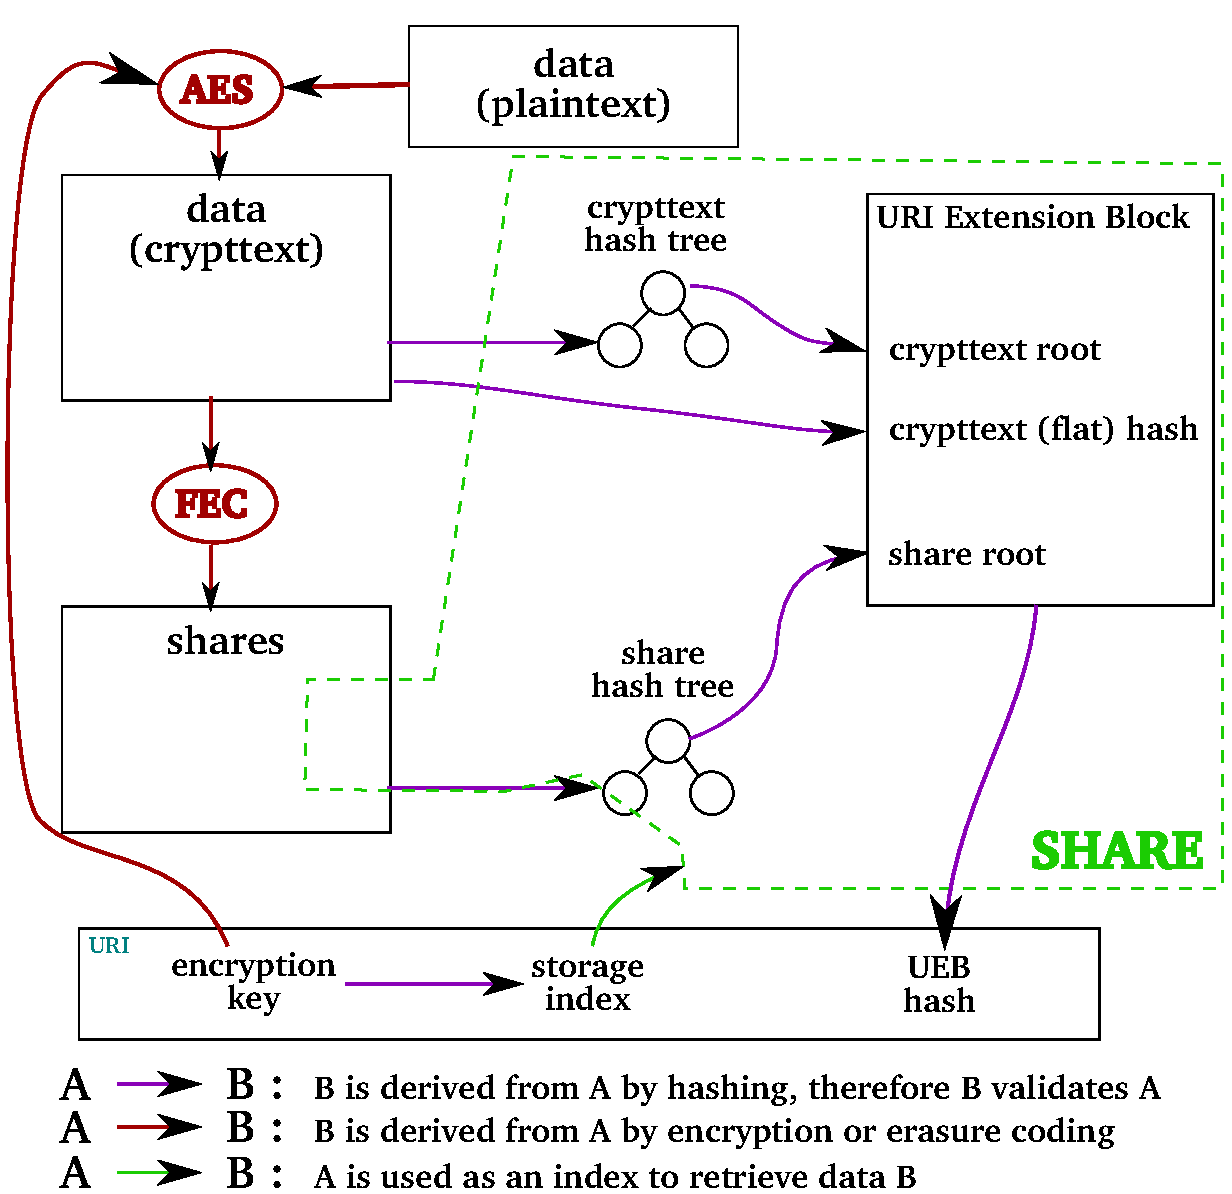
\includegraphics[width=0.9\columnwidth]{Tahoe-hashes.pdf}
    \caption{Tahoe-LAFS: Example of hashing operations.}
    \label{fig:tahoehashing}
    \emph{Figure based on
     \href{http://tahoe-lafs.org/source/tahoe/trunk/docs/specifications/CHK-hashes.svg}
     {CHK-hashes.svg from Tahoe-LAFS documentation}}
\end{figure}

As seen in figure \ref{fig:tahoehashing}, the usage of secure hashing is
extensive in Tahoe, and has to be considered as a key part of the functionality,
and thus affecting the performance.

\paragraph{Hash Trees.}

\begin{figure}[h]
    \centering
    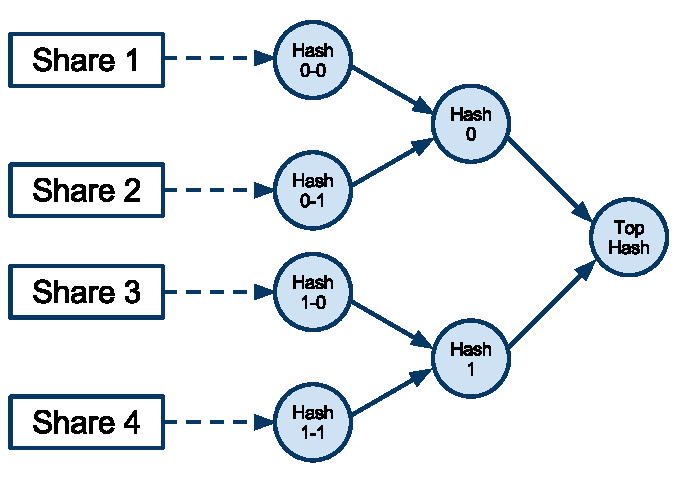
\includegraphics[width=0.9\columnwidth]{Tahoe-MerkleTree.pdf}
    \caption{Example of a Merkle tree.}
    \label{fig:tahoemerkletree}
\end{figure}

A hash tree, also known as a \emph{Merkle tree}, is a type of data structure
which can be described as a tree with nodes that can verify all information
below in the hierarchy, as depicted in figure \ref{fig:tahoemerkletree}. This
enables Tahoe to verify small segments of a file at the time, and this can be
used for instance to start playing a movie file while it is still being
downloaded.

These secure hashes of the shares of a file, are contained within a small
datastructure named the \emph{\ac{CEB}}.

\paragraph{Capabilities.}

A \textbf{capability} (or an URI) contains the encryption key, and a hash of the
\emph{\ac{UEB}}. The \ac{UEB} for each file is a data structure containing the
hash of the \ac{CEB}, the size of the file, any encoding parameters necessary to
perform the erasure decoding, and a hash of the plaintext and the encrypted
text. This is illustrated in figure \ref{fig:tahoeueb}.

\begin{figure}[!h]
    \centering
    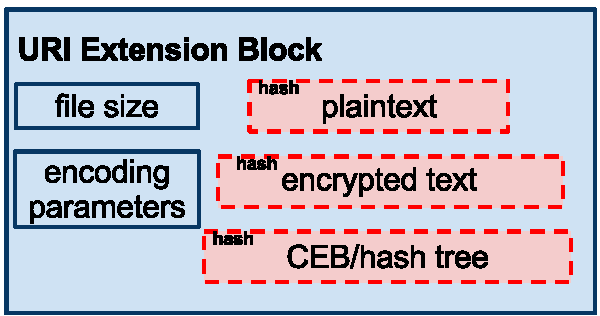
\includegraphics[width=0.9\columnwidth]{Tahoe-UEB.pdf}
    \caption{The composition of an \ac{UEB}.}
    \label{fig:tahoeueb}
\end{figure}

\paragraph{Storage Index.}

A hash of the encryption key is used to form the "storage index", which is
used for both server selection and to index shares within each storage node.
% More here?

\section{Python and Cython}
%What is it, how, why, alternatives?
% TODO: Finn en kilde på pythonting, om det trengs?
Python\footnote{\url{http://www.python.org/}} is a high-level general-purpose
programming language. Python is also an interpreted language, which means that
Python programs are compiled at runtime. There exists multiple implementations
of Python, however the most common, CPython, is implemented in C. The fact that
Python is a high-level language usually means that there are performance
penalties in contrast to lower level languages, such as C. To remedy this
problem it is possible to write extensions to the language by using the official
C-API. This approach has been used by several cryptographic libraries for
Python, such as pycryptopp\footnote{\url{http://tahoe-lafs.org/trac/pycryptopp}}
and the official hashlib\footnote{\url{http://code.krypto.org/python/hashlib/}}.

Tahoe-\ac{LAFS} is written in Python, but the SHA-3 candidate implementations found
in both the official NIST submissions and SUPERCOP are either in C or in
assembly. Therefore it is necessary to either implement the functions in Python
or make extensions to Python through the C-API, where extensions should give
the best performance.

\subsection{Cython}
Cython\footnote{\url{http://www.cython.org/}} is a language for writing Python
extensions in a language that closely resembles the Python language itself.
Basically what Cython does, is to parse Cython files and generate C source files
that utilises the Python C-API. Afterwards the generated source files can be
compiled as if they were written directly in C.

Direct calling of external C functions and methods is also supported, thus
making Cython an attractive way of wrapping external libraries written in C to
enable access from Python code.

Since the generation of C source files is an automated procedure, a small
performance trade-off is to be expected, due to the extra layer of abstraction.
The gain on the other hand, is significant in comparison to implementing
functions directly in Python.

%**************************************%
\chapter{Procedure}
%**************************************%

% FIXME: A more descriptive/better chapter title
%
%A bit more technical description of how we tested the candidates in Tahoe-LAFS
% - Limitations/assumptions
% - Optimized candidates.
% - Error sources.
% The points above should be taken into consideration on each section in this
% chapter.

In this chapter we will outline the procedure followed to complete our task.
% TODO: Mer intro

\section{Choosing implementations of the SHA-3 Candidates}

While the official \ac{NIST} \ac{SHA}-3 second round submissions contain both
a reference version and optimized versions of the candidates, it does not
appear to be updated since the submission deadline on September 15, 2009. They
also do not contain any benchmarking utility which could be used to decide on
the best implementation for a particular platform or architecture. \ac{SUPERCOP}
on the other hand, provides both, in combination with results stating which
compiler arguments gives the best performance. On the downside, the
\ac{SUPERCOP} \ac{API} only specifies the \texttt{crypto\_hash()} function and
not an \texttt{update()} function which Tahoe-\ac{LAFS} is dependent on using.

Since Tahoe-\ac{LAFS} is using \ac{SHA}-256 internally, we only test \ac{SHA}-3
functions with 256-bit output in our implementation. 


\subsection{Criteria for implementation selection}

We chose the fastest implementation of each candidate that conforms to the
following criteria:
\begin{enumerate}
  \item The implementation must have an \ac{API} defined in C.
  \item The implementation must include a working \verb update() function.
  \item The implementation must not use assembly that can not be made
    position independent by \ac{GCC}.
  \item The implementation should conform to the \acp{KAT} specified in the
    \ac{NIST} submission package, or later updates by the author.
\end{enumerate}

% TODO fix kilde
Based on these criteria, we choose the fastest possible implementation based
on our benchmark in \ac{SUPERCOP}. The relative speed of each implementation, in
relation to other implementation for the same and other candidates are
available at source.

\subsection{Chosen implementations}

\begin{table}
  \centering
  \begin{tabular}{ | l | l | l | }
    \hline
    \textbf{candidate} & \textbf{from} & \textbf{implementation} \\ \hline
     blake      & supercop-20101014 & blake32/ssse3 \\ \hline
     bmw        & supercop-20101014 & bmw256/optc01 \\ \hline
     cubehash   & sphlib 2.1        & c/cubehash.c  \\ \hline
     echo       & supercop-20101014 & echo256/sphlib\\ \hline
     fugue      & supercop-20101014 & fugue256/sphlib\\ \hline
     groestl    & supercop-20101014 & groestl256/sphlib\\ \hline
     hamsi      & supercop-20101014 & hamsi/simd-1  \\ \hline
     jh         & supercop-20101014 & jh256/sphlib  \\ \hline
     keccak     & supercop-20101014 & keccakc512/sseu2 \\ \hline
     luffa      & supercop-20101014 & luffa256/sse2 \\ \hline
     shabal     & supercop-20101014 & shabal256/sphlib\\ \hline
     shavite3   & supercop-20101014 & shavite3256/no-salt       \\ \hline
     simd       & supercop-20101014 & simd256/vect128 \\ \hline
     skein      & supercop-20101014 & skein256/opt           \\ \hline
  \end{tabular}
  \caption{Choosen \ac{SHA}-3 candidate implementations}
  \label{tbl:sha3:implementations}
\end{table}


The chosen implementations are shown in Table \ref{tbl:sha3:implementations}
and their compiler flags used, which are extracted from the \ac{SUPERCOP}
results can be seen in Table\ref{tbl:sha3:compilerflags}. It should be noted
that 32 in blake32 does not refer to the output length of the function, but the
fact that the algorithm is optimized for 32-bit usage. 512 in Keccackc512 also
does not mean 512-bit output, but 512 cycles in the internal function. The
relative speeds of the implementations chosen compared to the best version in
\ac{SUPERCOP} and relative speed of the benchmark compared to other candidates
can bee seen in Table \ref{tbl:sha3:speedrelative}. It should also be noted
that the fastest sha256 implementation in \ac{SUPERCOP} is
cryptopp\footnote{\url{http://www.cryptopp.com/}}, which is the one used by
Tahoe-\ac{LAFS}. For the most part we have found working versions of all
candidates in \ac{SUPERCOP}, however there are some exceptions. 

\begin{table}
  \centering
  \begin{tabular}{ | l | l | }
    \hline
    \textbf{Candidate} & \textbf{Compiler flags}            \\ \hline
     BLAKE       & -m32 -march=native -mtune=native -O      \\ \hline
     \ac{BMW}    & -funroll-loops -m32 -march=pentium4 -O3  \\ \hline
     Cubehash    & -O2                                      \\ \hline
     Echo        & -funroll-loops -m32 -march=prescott -O2  \\ \hline
     Fugue       & -funroll-loops -O                        \\ \hline
     Grøstl      & -m32 -march=pentium3 -O                  \\ \hline
     Hamsi       & -funroll-loops -m32 -march=pentium-m -O3 \\ \hline
     JH          & -m32 -march=core2 -O                     \\ \hline
     Keccak      & -march=barcelona -O3                     \\ \hline
     Luffa       & -funroll-loops -march=k8 -O3             \\ \hline
     Shabal      & -funroll-loops -m32 -march=pentium2      \\ \hline
     Shavite3    & -funroll-loops -march=i486 -O            \\ \hline
     Simd        & -m32 -march=barcelona -O2                \\ \hline
     Skein       & -march=pentium2 -O2                      \\ \hline
  \end{tabular}
  \caption{GCC compiler flags used on the implementations}
  \label{tbl:sha3:compilerflags}
\end{table}


\begin{table}
  \centering
  \caption{Chosen SHA-3 implementations relative performance}
  \begin{tabular}{ | l | p{6cm} | r | }
    \hline
    \textbf{Candidate} & \textbf{Relative speed compared to fastest implementation} \\ \hline
     BLAKE      & 1.00                   \\ \hline
     Shabal     & 1.46                   \\ \hline
     \ac{BMW}   & 1.46                   \\ \hline
     Simd       & 1.00                   \\ \hline
     Luffa      & 1.12                   \\ \hline
     Fugue      & 2.03                   \\ \hline
     Keccak     & 1.00                   \\ \hline
     Hamsi      & 1.00                   \\ \hline
     Skein      & 2.18                   \\ \hline
     Echo       & 1.48                   \\ \hline
     Grøstl    & 3.09                   \\ \hline
     JH         & 6.19                   \\ \hline
     Shavite3   & unknown                \\ \hline
     Cubehash   & unknown                \\ \hline
  \end{tabular}
  \label{tbl:sha3:speedrelative}
\end{table}


\paragraph{JH} seems to be broken in every implementation with regard to
criteria 2. For both the optimized versions found in \ac{SUPERCOP} and the
reference implementations in the \ac{NIST} submission package, Hash("foofoo")
will not yield the same result as two consecutive calls to Update("foo").
However the implementation in sphlib does fulfill this requirement. We have
also contacted the author, Thomas Pornin, which confirms this problem with the
official JH candidate and that the author has been made aware of the problem
but has not released any updated version yet.
% TODO: Fix hvordan vi referer til e-post?

\paragraph{Cubehash} sadly does not have a version in \ac{SUPERCOP} with a 256-bit
output, which is why we have only included a version from sphlib.

\paragraph{Simd vect128 implementation} does not by default conform to
criteria 4, because of a bug in the implementation. This has confirmed by the
author who also supplied us with a patch to correct the bug.

\paragraph{Blake32 \ac{SSSE3}} implementation also fail to wholly fulfill
criteria 4, however it does validate all test vectors that have a length 
in bits which is a multiple of 8. Since our Python wrappers only allow, and
only need, to provide data in full bytes we decided to keep this
implementation.

\paragraph{Shavite3} seems to have received an update\footnote{see
\url{http://www.cs.technion.ac.il/~orrd/SHAvite-3/}}. We have observed that
implementations of Shavite3 in \ac{SUPERCOP}-20101014 or later seems to fail to
verify the \ac{KAT}s, while the version we have used does. We believe this is
only because newer \ac{KAT}s will have to be generated, but since the author
has not done so we chose to use an older version of the algorithm.

% TODO: Add some lines that give reasons for the criteria above.

% sphlib, SUPERCOP, NIST

\section{Python bindings}

Since Tahoe-\ac{LAFS} is written in Python, we needed some way of interacting
with the C implementations of the NIST candidates. We did this by the use of
Cython, and built a python object-oriented library which we named SHA3lib.
SHA3lib supports all of the 14 second round \ac{SHA}-3 candidates, but only in
their 256-bit form.

\subsection{SHA3lib}
SHA3lib is built to mimic the functionality of
hashlib\footnote{\url{http://docs.python.org/library/hashlib.html}}, the
default python library for MD5, \ac{SHA}-1 and the \ac{SHA}-2 family. 
% TODO, figure or listing of what this means

\subsubsection{Cython}
We employ Cython to generate bindings for the C implementation and the
different candidates, as well as to create the base python classes. To access
functions in C we need to generate a Cython header file, which pretty much does
the same as a C header file; it tells which functions and data types are
available. How we accomplish this for an implementation that satisfies the
\ac{NIST} \ac{API} is shown in Listing \ref{lst:cython_header}. 

\begin{lstlisting}[label=lst:cython_header, caption=Cython header\, echo\_hash\_h.pxd]
cdef extern from "sha3nist.h":
    ctypedef unsigned char BitSequence
    ctypedef unsigned long long DataLength

    cdef enum HashReturn:
        SUCCESS = 0
        FAIL = 1
        BAD_HASHLEN = 2

    ctypedef struct hashState:
        pass

    HashReturn Hash(int, BitSequence *data, 
                    DataLength, 
                    BitSequence *hashval)
    HashReturn Init(hashState *state, 
                    int hashbitlen)
    HashReturn Update(hashState *state, 
                      BitSequence *data, 
                      DataLength databitlen)
    HashReturn Final(hashState *state, 
                    BitSequence *hashval)
\end{lstlisting}

We then create a wrapper-class that mimics hashlib, this is shown in Listing
\ref{lst:cython_impl}. Functions declared with def er python functions, cdef are
Cython only while cpdef are functions that can be accessed from both. While
this is just the implementation for the echo candidate, the almost exact same
pattern is used for all of the other candidates. 

\begin{lstlisting}[label=lst:cython_impl, caption=Cython class\, echo\_hash.pyx]
cimport echo_hash_h
cimport cython

from libc.stdlib cimport *

cdef class echo:
    '''
    A class that tries to mimic the behaviour of hashlib, 
    i.e.  keeping state so that one can update the hashing 
    procedure instead of doing it from scratch.
    '''
    cdef echo_hash_h.hashState previous_state
    cdef echo_hash_h.hashState state
    cdef int finished
    cdef int hashbitlen
    cdef list hashval

    def __init__(self, int in_hashbitlen, 
                 bytes initial=None):
        self.finished = 0
        self.hashbitlen = in_hashbitlen
        echo_hash_h.Init(&self.state, self.hashbitlen)

        if initial:
            self.update(initial)

    cpdef update(self, bytes in_data):
        cdef char* data = <char *> in_data
        cdef int data_len = len(in_data)*8

        if self.finished:
            self.finished = 0
            self.state = self.previous_state

        echo_hash_h.Update(&self.state, 
                        <echo_hash_h.BitSequence *> data, 
                        data_len)

    cpdef final(self):
        cdef echo_hash_h.BitSequence *hashval = \
        <echo_hash_h.BitSequence *> \
        malloc(self.hashbitlen*8)

        # We copy the state so that we can continue to 
        # update. This equals hashlibs functionality, 
        # but not pycryptopp.
        self.previous_state = self.state

        echo_hash_h.Final(&self.state, hashval)
        self.finished = 1

        self.hashval = [hashval[i] for i from 0 <= i \
                        < self.hashbitlen / 8]
        free(hashval)

    cpdef copy(self):
        s = echo(self.hashbitlen)
        s.state = self.state
        s.previous_state = self.previous_state
        s.finished = self.finished
        if s.finished:
            s.hashval = self.hashval

        return s

    def digest(self):
        if not self.finished:
            self.final()

        return ''.join(map(chr, self.hashval))

    def hexdigest(self):
        if not self.finished:
            self.final()

        return ''.join(['%02x' % i for i in self.hashval])
\end{lstlisting}

\subsubsection{\ac{Distutils}} We use the
\ac{Distutils}\footnote{\url{http://docs.python.org/distutils/}} to build and
install our code. The alternative to doing this would be to manually transform
cython files to C-files, build the shared library from this and other relevant
C-files and then install by copying into the correct system directory where
python libraries should be stored. \ac{Distutils} also support expansion
through self defined commands, something we have utilised to do Unit Testing.
Options and configuration for \ac{Distutils} is done through a file setup.py.
Relevant configuration for compiling the echo extension, and installing SHA3lib
can bee seen in Listing \ref{lst:setup_py}.


\begin{lstlisting}[label=lst:setup_py, caption=Compiling echo from \ac{Distutils}]
from distutils.core import setup, Command
from distutils.extension import Extension
from Cython.Distutils import build_ext

srcpath = 'sha3lib/'
hashpath = srcpath + 'hash_functions/'

ext_modules = [
    Extension("sha3lib.hash_functions.echo.echo_hash",
        [hashpath+"echo/echo_hash.pyx", 
         hashpath+'echo/sha3nist.c', 
         hashpath+"echo/echo.c"],
    extra_compile_args=[
        '-funroll-loops',
        '-m32',
        '-march=prescott',
        '-O2',
        '-fomit-frame-pointer']
    ),
]

setup(
    name='SHA3lib',
    version='0.1',
    description='Python bindings for SHA3-256 using Cython',
    cmdclass = {'build_ext': build_ext},
    ext_modules = ext_modules,
    packages =
        ['sha3lib',
        'sha3lib.hash_functions',
        'sha3lib.hash_functions.echo',],
)

\end{lstlisting}



\subsection{Unit tests}
% Include the use of Known Answer Tests

\section{Modifications in the Tahoe-\ac{LAFS} Code}

The code of Tahoe-LAFS conforms to the style guide of Python, known as PEP 8.
This, along with the code being highly modular and consistent to its
architecture, emphasizes code readability.
With some experience using Python, it is not difficult to learn the Tahoe code
enough to understand what is happening when a file is uploaded or downloaded
with the system.

All hashing operations requested by the Tahoe system is routed through a
couple of classes and functions, and the connection to the underlying hash
function library is made on only one line. This is displayed in Listing
\ref{lst:hashutil}.

\begin{lstlisting}[label=lst:hashutil, caption=Extract from hashutil.py of Tahoe-LAFS source.]
from pycryptopp.hash.sha256 import SHA256
...
class _SHA256d_Hasher:
    ...
    def __init__(self, truncate_to=None):
        self.h = SHA256()
        self.truncate_to = truncate_to
        self._digest = None

    def update(self, data):
        assert isinstance(data, str) # no unicode
        self.h.update(data)

    def digest(self):
        if self._digest is None:
            h1 = self.h.digest()
            del self.h
            h2 = SHA256(h1).digest()
            if self.truncate_to:
                h1 = h1[:self.truncate_to]
                h2 = h2[:self.truncate_to]
            self._digest = h2

        return self._digest
\end{lstlisting}

As stated in Section \ref{sec:lengthextension}, none of the SHA-3 candidates is
vulnerable to the length-extension attack. Since we are interested in finding
out how Tahoe-\ac{LAFS} performs when utilizing the SHA-3 functions, we can
remove the lines that fixes the length-extension problems manually. In addition,
to try out one of the new implementations, we change line one in Listing
\ref{lst:hashutil}, and an example of this can be seen in Listing
\ref{lst:hashutilmod}.

\begin{lstlisting}[label=lst:hashutilmod, caption=Relevant parts of hashutil.py of Tahoe-LAFS source after modification.]
from sha3lib import bmw256 as SHA256
...
class _SHA256d_Hasher:
    ...
    def __init__(self, truncate_to=None):
        self.h = SHA256()
        self.truncate_to = truncate_to
        self._digest = None

    def update(self, data):
        assert isinstance(data, str) # no unicode
        self.h.update(data)

    def digest(self):
        if self._digest is None:
            h1 = self.h.digest()
            del self.h
            if self.truncate_to:
                h1 = h1[:self.truncate_to]
            self._digest = h1

        return self._digest
\end{lstlisting}

Some notes has to be made regarding the first line in Listing
\ref{lst:hashutilmod}. For every candidate we test, the whole setup and grid is
started from ground up, since changing the hash function this way cause a
backwards compatibility break, making it impossible to download files put to the
grid while using another hash function.
For the same reasons, some of the built-in unit tests of Tahoe-LAFS fail when
changing this line, because they contain test fixtures made with SHA-256.
This also renders uploading of mutable files impossible, since the internal
verification fails. For this reason, \emph{only immutable files} are tested and
measured in this paper.

\section{Test vectors and Configuration}

% TODO: Write something about why we only test the client

\section{Distribution of the Code}
% Distutil, bash scripts

%**************************************%
\chapter{Measurements and Results}
%**************************************%

% Maybe cite
% \url{http://tahoe-lafs.org/trac/tahoe-lafs/wiki/Performance?version=32}


\subsection{\ac{SUPERCOP} benchmarks}
The results of \ac{SHA}-3
256-bit functions and \ac{SHA}-256 benchmarking in \ac{SUPERCOP} can be seen in
tables \ref{tbl:supercop:long}, \ref{tbl:supercop:4096},
\ref{tbl:supercop:1536}, \ref{tbl:supercop:576}, \ref{tbl:supercop:64} and
\ref{tbl:supercop:8}. The lower the numbers, the faster the algorithms
performed in the test.

\begin{table}
  \centering
  \begin{tabular}{ | c | c | c | l | }
    \hline
    \textbf{Quartile} & \textbf{Median} & \textbf{Quartile} & \textbf{Function} \\ \hline
    6.01 & 6.01 & 6.02 & shabal256 \\ \hline
    6.91 & 6.94 & 7.18 & bmw256 \\ \hline
    8.37 & 8.38 & 8.43 & blake32 \\ \hline
    11.13 & 11.15 & 11.23 & simd256 \\ \hline
    13.53 & 13.53 & 13.53 & luffa256 \\ \hline
    15.45 & 15.46 & 15.50 & sha256 \\ \hline
    17.54 & 17.64 & 17.71 & fugue256 \\ \hline
    18.10 & 18.61 & 18.62 & skein256 \\ \hline
    18.95 & 18.96 & 18.98 & jh256 \\ \hline
    20.40 & 20.88 & 20.92 & keccakc512 \\ \hline
    23.36 & 23.47 & 23.48 & groestl256 \\ \hline
    29.84 & 29.96 & 30.19 & hamsi \\ \hline
    32.21 & 32.25 & 32.34 & shavite3256 \\ \hline
    32.62 & 32.64 & 32.66 & echo256 \\ \hline
  \end{tabular}
  \caption{Results from SUPERCOP: Cycles/byte for long messages}
  \label{tbl:supercop:long}
\end{table}

\begin{table}
  \centering
  \caption{Results from SUPERCOP: Cycles/byte for 4096 bytes}
  \begin{tabular}{ | c | c | c | l | }
    \hline
    \textbf{Quartile} & \textbf{Median} & \textbf{Quartile} & \textbf{Function} \\ \hline
    6.44 & 6.44 & 6.44 & shabal256 \\ \hline
    7.28 & 7.29 & 7.37 & bmw256 \\ \hline
    8.58 & 8.58 & 8.60 & blake32 \\ \hline
    11.52 & 11.52 & 11.53 & simd256 \\ \hline
    13.87 & 13.87 & 13.87 & luffa256 \\ \hline
    15.82 & 15.83 & 15.84 & sha256 \\ \hline
    18.46 & 18.63 & 18.63 & skein256 \\ \hline
    19.27 & 19.28 & 19.31 & fugue256 \\ \hline
    19.32 & 19.32 & 19.32 & jh256 \\ \hline
    21.32 & 21.49 & 21.50 & keccakc512 \\ \hline
    24.11 & 24.16 & 24.16 & groestl256 \\ \hline
    30.11 & 30.14 & 30.22 & hamsi \\ \hline
    32.76 & 32.77 & 32.77 & echo256 \\ \hline
    32.87 & 32.89 & 32.92 & shavite3256 \\ \hline
  \end{tabular}
  \label{tbl:supercop:4096}
\end{table}

\begin{table}
  \centering
  \begin{tabular}{ | c | c | c | l | }
    \hline
    \textbf{quartile} & \textbf{median} & \textbf{quartile} & \textbf{hash} \\ \hline
    7.18 & 7.18 & 7.19 & shabal256 \\ \hline
    7.59 & 7.71 & 7.82 & bmw256 \\ \hline
    8.91 & 8.92 & 8.92 & blake32 \\ \hline
    11.86 & 11.87 & 11.89 & simd256 \\ \hline
    14.43 & 14.43 & 14.64 & luffa256 \\ \hline
    16.44 & 16.45 & 16.45 & sha256 \\ \hline
    18.80 & 18.96 & 18.97 & skein256 \\ \hline
    19.89 & 19.90 & 19.91 & jh256 \\ \hline
    21.96 & 21.98 & 22.03 & fugue256 \\ \hline
    22.31 & 22.31 & 22.36 & keccakc512 \\ \hline
    25.27 & 25.28 & 25.29 & groestl256 \\ \hline
    30.36 & 30.39 & 30.60 & hamsi \\ \hline
    33.93 & 33.93 & 33.94 & shavite3256 \\ \hline
    35.90 & 35.91 & 35.95 & echo256 \\ \hline
  \end{tabular}
  \caption{Results from SUPERCOP: Cycles/byte for 1536 bytes}
  \label{tbl:supercop:1536}
\end{table}

\begin{table}
  \centering
  \caption{Results from SUPERCOP: Cycles/byte for 576 bytes}
  \begin{tabular}{ | c | c | c | l | }
    \hline
    \textbf{Quartile} & \textbf{Median} & \textbf{Quartile} & \textbf{Function} \\ \hline
    8.82 & 8.88 & 9.02 & bmw256 \\ \hline
    9.12 & 9.16 & 9.21 & shabal256 \\ \hline
    9.80 & 9.81 & 9.86 & blake32 \\ \hline
    12.91 & 12.97 & 13.00 & simd256 \\ \hline
    15.85 & 15.86 & 16.04 & luffa256 \\ \hline
    17.99 & 18.05 & 18.08 & sha256 \\ \hline
    19.95 & 19.95 & 19.97 & skein256 \\ \hline
    21.47 & 21.49 & 21.52 & jh256 \\ \hline
    25.09 & 25.12 & 25.22 & keccakc512 \\ \hline
    28.23 & 28.26 & 28.26 & groestl256 \\ \hline
    29.16 & 29.25 & 29.38 & fugue256 \\ \hline
    30.84 & 30.94 & 30.96 & hamsi \\ \hline
    36.73 & 36.76 & 36.79 & shavite3256 \\ \hline
    42.85 & 42.87 & 42.88 & echo256 \\ \hline
  \end{tabular}
  \label{tbl:supercop:576}
\end{table}

\begin{table}
  \centering
  \caption{Results from SUPERCOP: Cycles/byte for 64 bytes}
  \begin{tabular}{ | c | c | c | l | }
    \hline
    \textbf{Quartile} & \textbf{Median} & \textbf{Quartile} & \textbf{Function} \\ \hline
    21.25 & 21.25 & 21.66 & blake32 \\ \hline
    23.77 & 23.78 & 24.17 & bmw256 \\ \hline
    26.44 & 26.56 & 26.83 & simd256 \\ \hline
    32.41 & 32.53 & 32.55 & skein256 \\ \hline
    33.47 & 33.59 & 33.73 & luffa256 \\ \hline
    34.92 & 35.06 & 35.20 & shabal256 \\ \hline
    38.11 & 38.12 & 38.64 & sha256 \\ \hline
    40.11 & 40.38 & 40.38 & hamsi \\ \hline
    40.25 & 40.38 & 40.91 & jh256 \\ \hline
    50.20 & 50.34 & 50.47 & keccakc512 \\ \hline
    64.94 & 65.08 & 65.34 & groestl256 \\ \hline
    72.91 & 73.05 & 73.31 & shavite3256 \\ \hline
    101.20 & 101.33 & 101.47 & echo256 \\ \hline
    123.11 & 123.91 & 125.38 & fugue256 \\ \hline
  \end{tabular}
  \label{tbl:supercop:64}
\end{table}

\begin{table}
  \centering
  \begin{tabular}{ | c | c | c | l | }
    \hline
    \textbf{Quartile} & \textbf{Median} & \textbf{Quartile} & \textbf{Function} \\ \hline
    107.25 & 107.38 & 108.38 & blake32 \\ \hline
    114.75 & 117.88 & 119.00 & hamsi \\ \hline
    131.75 & 132.88 & 136.00 & bmw256 \\ \hline
    145.50 & 145.62 & 151.88 & luffa256 \\ \hline
    177.50 & 179.62 & 180.62 & sha256 \\ \hline
    183.88 & 184.88 & 184.88 & skein256 \\ \hline
    215.75 & 218.88 & 227.38 & simd256 \\ \hline
    226.38 & 229.50 & 232.62 & shabal256 \\ \hline
    328.25 & 329.38 & 330.38 & jh256 \\ \hline
    329.38 & 329.38 & 331.50 & shavite3256 \\ \hline
    337.88 & 339.00 & 340.00 & groestl256 \\ \hline
    399.50 & 401.62 & 404.88 & keccakc512 \\ \hline
    807.50 & 807.50 & 808.62 & echo256 \\ \hline
    855.38 & 862.75 & 874.50 & fugue256 \\ \hline
  \end{tabular}
  \caption{Results from SUPERCOP: Cycles/byte for 8 bytes}
  \label{tbl:supercop:8}
\end{table}


What is tested and what is not tested?

How much time is spent on hashing versus upload over network?

How much gain can Tahoe-LAFS get by switching to SHA-3?

Plenty of tables, graphs

%**************************************%
\chapter{Discussion}
%**************************************%

What could have been done differently?

Compare results with general (supercop) results.

Optimized candidates.

%**************************************%
\chapter{Conclusion and Future Work}
%**************************************%

A somewhat short conclusion summing up what has been done, and results and
discussion

New SHA-3 capability in Tahoe-LAFS (GSOC ref) to get our code to trunk


% BibTeX bibliography lives in external file
\bibliographystyle{plainnat}
\bibliography{ref_sha3,ref_tahoe}

% Uncomment to enable appendices.
%\appendix
%\appendixpage
%\addappheadtotoc

% Use ordinary \chapters from here on..

\end{document}
